\chapter{Introduction}\label{ch:introduction}
\graphicspath{{../Figures/10-introduction/}{figs/10-introduction/}}

\section{Motivation}

Biomimetic robots provide a platform for investigating how mechanical structure and control interact to generate movement, offering complementary insights to simulation-based studies \citep{andrews_general_1985, millard_flexing_2013, arnold_model_2010}. Wheeled robots remain the platform of choice in structured environments, where their speed, efficiency, and payload capacity are difficult to match; in the unstructured terrain of the natural and built world, legged machines hold the advantage, and biomimetic legs that reproduce human force capabilities have the potential to excel where wheels cannot \citep{frey_legged_2026, ha_learning_2025}. Musculoskeletal humanoids and limb systems driven by tendon-like actuators have been shown to support biologically meaningful experiments on motion generation, internal force transmission, and neural control hypotheses \citep{asano_design_2017, asano_musculoskeletal_2019, hitzmann_anthropomorphic_2018, liu_robotic_2018, chen_realizing_2019}. The dual perspective of using robots to learn about biology, and using biology to design more adaptive robots, has been emphasized in both biomimetic robotics and biomechanics \citep{ijspeert_amphibious_2020, asano_design_2017}. With such robotic systems, experiments can be performed that would not be practical or ethical with human test subjects, such as removing a specific muscle from the system or blocking a sensory feedback pathway. Experiments of this kind allow direct testing of how the components of the neuromechanical system interact, and they offer new opportunities for testing neural control theories that are faster and cheaper than human observation studies \citep{shin_constructive_2018, goldsmith_investigating_2021, schilling_adaptive_2022}.

Artificial muscles are a key enabling technology for this class of robot. Among the available actuation technologies, McKibben-style braided pneumatic actuators (BPAs) combine low mass, high force-to-weight ratio, and intrinsic compliance with a force--length curve that qualitatively resembles that of skeletal muscle \citep{liang_comparative_2020, hunt_modeling_2017}. BPAs have been used in quadrupedal robots \citep{aschenbeck_design_2006, hunt_modeling_2017, scharzenberger_design_2019}, musculoskeletal humanoids \citep{asano_design_2017, hitzmann_anthropomorphic_2018}, and dexterous manipulation systems \citep{chen_realizing_2019}. However, BPAs also differ from biological muscle in important ways: their maximum tensile force occurs at resting length rather than at an optimal fiber length, their maximum contraction ratio is substantially lower than that of human muscle, and their force output is a highly nonlinear function of internal pressure, contraction, and loading state \citep{hunt_modeling_2017, sarosi_comparative_2017, liang_comparative_2020}. My experience with \qty{10}{\mm} actuators made this gap concrete: manufacturer specifications overstate the force and contraction available at the short resting lengths a leg design requires, and designs based on those specifications delivered less range of motion and joint torque than intended. Nor could the published empirical models fill in the gaps, because each is fitted to measurements at a single resting length \citep{sarosi_comparative_2017, martens_modeling_2017, hunt_modeling_2017}; none accurately predicts how force changes when a designer chooses a different actuator length. Because muscle resting length is one of the primary degrees of freedom available to the robot designer, the absence of a force model valid at arbitrary resting length blocked accurate actuator selection. Designing a biomimetic robot around BPAs therefore requires quantitative, predictive models of the actuator and of the joint torques it can produce.

Actuator force alone, however, does not determine the torque a joint produces. The robot knee transmits BPA force to the skeleton through mounting brackets, artificial tendons, and paths that wrap over the joint, and each of these elements departs from the rigid-body idealization: brackets and fixtures deflect under load, tendons stretch, and a wrapping actuator loses usable length as the knee flexes. At the start of this work it was unknown how much these transmission effects reduce the torque delivered at the knee relative to the rigid-body prediction, and no method existed for correcting that prediction in a form that would transfer between joint configurations. The biomimetic knee's optimized muscle routing \citep{morrow_optimization_2020} compounded the problem: it had never been validated experimentally or compared against human isometric torque data, so even the nominal torque envelope of the robot leg rested on unverified calculations.

Researchers implementing neural control models face two related problems. Sensory-afferent findings are distributed across species, preparations, and experimental protocols, so selecting a feedback pathway requires locating its measured properties and the conditions under which they were observed \citep{van_de_crommert_review_1998, windhorst_muscle_2007, windhorst_spinal_2022}. I addressed that evidence-access problem with the Sensory Afferent Database. A second problem arises when a published neural circuit is coupled to a different mechanical model: its behavior depends on the actuator mechanics, sensory signals, support conditions, and numerical implementation as well as on the circuit itself. Published architectures and software supply essential components \citep{rybak_modelling_2006, mccrea_organization_2008, markin_afferent_2010, nourse_sns_2023}, but the behavior of their particular combination must be established. I developed coupled human and artificial-muscle models, graphical neural blocks, and controlled evaluation procedures to distinguish these contributions. Representative tests establish circuit agreement across implementations, corrective reflex behavior, and the dependence of a supported stepping configuration on selected feedback pathways.

The dissertation therefore addresses four connected needs: an actuator-force model that accounts for resting length, corrections for transmission losses at the knee, a curated sensory-afferent resource, and tools for developing and checking neuromechanical simulations. Together, they support the design and evaluation of the robot; achieving unsupported walking remains a separate control and integration problem.

\section{The Biomimetic Humanoid Robot Project}\label{sec:project}

This dissertation is part of a long-running effort at Portland State University to build a biomimetic humanoid robot from the trunk down, actuated by pneumatic artificial muscles and controlled by a synthetic nervous system (SNS). The project is deliberately iterative. Knowledge from biomechanics and neuroscience guides the design of robots intended to perform complex tasks in unstructured environments with improved efficiency, balance, adaptability, and resilience. Those robots then become physical models with which biological hypotheses can be tested, validated, and refined through controlled changes that would be impractical or unethical in living subjects. The resulting biological insight informs the next generation of robot design, and lessons from both directions can be translated into improved prosthetic and orthotic devices.

The present work builds directly on a series of studies by me and my collaborators. In my master's project, the kinematics and dynamics of a biomimetic robot leg were matched against the Gait2392 OpenSim model, artificial muscle attachment and wrapping locations were determined for the robot legs, and MATLAB software was developed for evaluating muscle lengths, moment arms, and isometric joint torques over the full range of motion \citep{bolen_bipedal_2019, bolen_determination_2019}. That work showed that simply transplanting human muscle attachment locations onto a BPA-actuated robot does not reproduce human torque profiles; the placement optimization that closes this gap was completed during this dissertation and is summarized in Section~\ref{sec:foundation}. The rest of the platform advanced in parallel, and this dissertation builds on its hardware and demonstrations: the biomimetic four-bar knee linkage with a migrating instantaneous center of rotation, designed and validated by Steele \citep{steele_development_2017, steele_biomimetic_2018, steele_biomimetic_2018-1}, is the knee of the robot leg whose torque transmission Chapter~\ref{ch:torque} measures, and the canine-inspired quadruped platform Muscle Mutt, formerly called DoggyDeux, demonstrated antagonistic BPA pairs under synthetic nervous system control on a physical robot \citep{scharzenberger_design_2019}, extending an earlier AARL demonstration of central pattern generator control of a pneumatically actuated robot \citep{hunt_development_2017}. The humanoid leg of this dissertation carries that line forward.

\section{Research Objectives}\label{sec:objectives}

This dissertation investigates actuator force and knee torque experimentally, consolidates sensory-afferent evidence in the Sensory Afferent Database \citep{bolen_sensory_2023, bolen_using_2024}, and develops neural-model and simulation interfaces with representative verification checks. The objectives are:

\begin{enumerate}
    \item \textbf{Characterize the isometric force of Festo BPAs} with uninflated diameters of \qtylist{10;20}{\mm} over a wide range of resting lengths, contractions, and pressures; derive improved maximum-force and normalized force--strain--pressure models; and compare them against existing models (Chapter~\ref{ch:muscles}).
    \item \textbf{Validate and improve the prediction of isometric knee torque} produced by BPAs on pinned-joint and biomimetic four-bar knees; identify and model losses caused by constant length offsets, series compliance, and actuator wrapping; and compare the resulting torque envelopes with human capabilities (Chapter~\ref{ch:torque}).
    \item \textbf{Consolidate the sensory afferent literature into a structured afferent resource}, the Sensory Afferent Database, by auditing and curating the published record of afferent properties across animal species and their role in motor control, and by evaluating AI-assisted literature triage for expanding the corpus (Chapter~\ref{ch:database}).
\item \textbf{Develop and demonstrate neuromechanical modeling tools} by implementing the Li--Deng walker, Gait2392-based models with alternative neural controllers and artificial-muscle actuation, SNS-Simscape blocks for neural pathways, and staged tuning and experiment procedures; verify representative circuit responses, implementation agreement, and neural--mechanical signal exchange (Chapters~\ref{ch:sns} and~\ref{ch:overall}).
\end{enumerate}

\section{Dissertation Organization}\label{sec:organization}

Chapter~\ref{ch:background} introduces the robot, BPA actuation, musculoskeletal design, locomotor control, and the scientific rationale for robotic models. Chapter~\ref{ch:muscles} presents the isometric force characterization and actuator models, adapted from my publication \citep{bolen_2026}. Chapter~\ref{ch:torque} tests the joint-torque predictions, identifies compliance and wrapping corrections, and uses them to redesign actuator routes.

Chapter~\ref{ch:database} presents the Sensory Afferent Database, its curation, and its use limits. Chapter~\ref{ch:sns} begins with the AnimatLab attempt to combine the Deng CPG and Li walker, identifies the development requirements exposed by that attempt, and presents the tools and representative checks built to address them. Chapter~\ref{ch:overall} discusses the contributions together and develops the future work; Chapter~\ref{ch:conclusion} states the conclusions. Figure~\ref{fig:roadmap} summarizes these connections.

\begin{figure}[htbp]
\centering
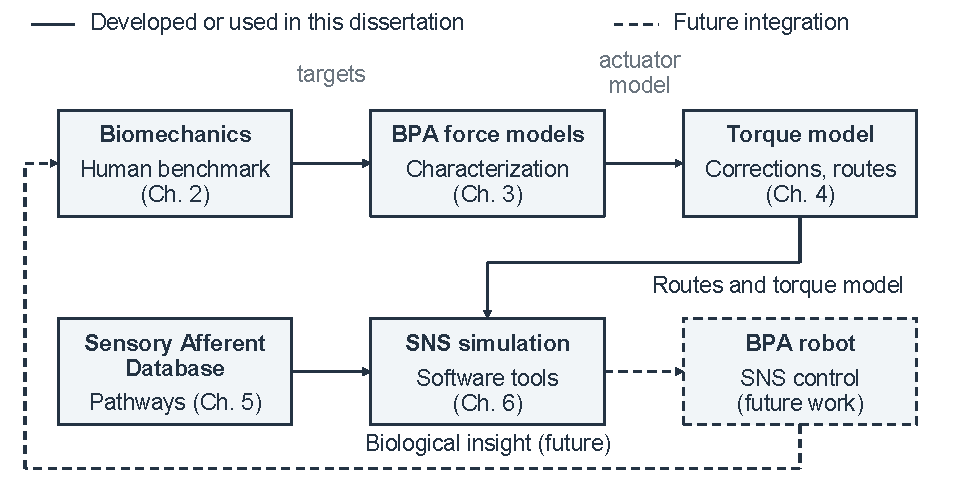
\includegraphics[width=\textwidth]{roadmap.pdf}
\caption[Dissertation roadmap]{Dissertation roadmap. Biomechanical targets guide actuator characterization and route design; the sensory-afferent resource informs feedback selection; and simulation tools support controller evaluation. Dashed connections indicate future integration and the intended return of biological insight.
}
\label{fig:roadmap}
\end{figure}

Appendices~\ref{app:muscle_calcs}--\ref{app:model_geometry} provide the muscle calculations, neural equations, model geometry, and supporting mechanical results. Appendix~\ref{app:simulation_verification} collects the larger simulation evaluations, and Appendix~\ref{app:sadb_records} provides the database coverage and pathway tables.